\section{Introduction}

With the current developments  in technology, Internet of Things(IoT) seems to have entered into every sphere of everyday life. From our homes to our cars to hospitals and other public and private institutions. Small heterogeneous embedded devices that are connected to each other wirelessly to provide services that were unimaginable before. However, the most important aspect of any service is to maintain security of the processed data and to maintain the privacy of the users. Hence the IoT services tend to implement dedicated security measures.\par
However, the Internet itself is evolving and now we see the advent of a new approach to the internet paradigm known as Information-centric networking (ICN). The new Internet concept revolves around the idea of not addressing the content on a particular device through IP addresses but through assigned name. The problem lies in the fact that IoT devices are very well expendable and to assign the myriad number of these devices with limited IP addresses and to create mappings on several routers is computationally expensive. These IP addresses have nothing to do with what content the device holds. It is only a unique identifier that is used by the network layer to communicate with other devices. \par
So what does this name-based addressing mean? The ICN infrastructure introduces the concept of naming the devices based on the content it holds or through the service it can access. This allows the data stored in any of these devices to become completely independent of the devices location, the application it is running on, the storage format, the means of transportation thereby reducing all these overheads of the data packet. The ICN favors the concept of caching and replication of data close to the service or the device where it is required. This allows for higher efficiency, better scalability and higher robustness of data in challenging communication scenarios. \par
This report discusses about how this ICN technology could be relevant for an IoT environment. We would see what features of ICN favor the networking in IoT devices. This will be discussed in the \ref{subsec: The Protocol stack in ICN}, where the ICN protocol stack will be discussed. Then we will discuss about the ICN middle-ware architecture that could potentially provide us with authenticity, confidentiality, integrity and privacy in \ref{subsec: IoT Middleware architecture} and thereafter the later sections will discuss with the help of UML diagrams, how these functionalities can be provided to our ICN-IoT system. \par
First and foremost,  ICN offers features such as caching, computing and storage, mobility, context-aware networking and support for ad hoc networking. Therefore it allows IoT devices a platform that supports device bootstrapping with minimal configuration, self organization capabilities of IoT elements and natural caching points in the network for faster retrieval of data.\par
Another aspect of ICN is that the data in this information-centric networking is delocalized and does not require retrieval via an end-to-end transport stream but instead with hop-wise replication and in-network caching, this facilitates information dissemination in the IoT environment, and relaxes the demand for continued connectivity.\par
These concepts can however be coupled with the existing Internet. ICN doesn't mean that Internet will be replaced, it only facilitates the features mentioned however it is easily implemented on top of the current IP infrastructure. The key point is that such a concept can be applied to different layers of the protocol stack to provide resource naming, ubiquitous caching and corresponding transport services. This naming functionalities would make fundamental changes in how the current routing and forwarding works.\par
 \begin{figure*}[ht]
	\centering
	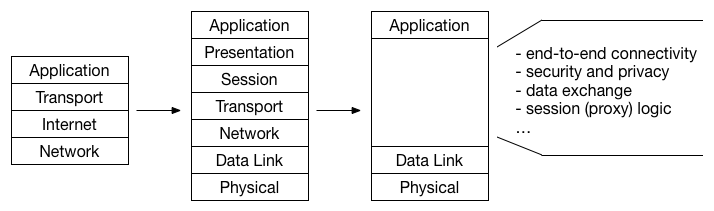
\includegraphics[width=0.8\linewidth]{Figures/tcpstack.png}
	\caption[]{TCP/IP stack}
	\label{fig:TCP/IP stack}
\end{figure*}
This being said, it is important to state that the current IP stack has a lot of overheads due to the increasing security measures it must implement. This reduces the overall efficiency and performance of the system. In order to combat that, ICN itself must be implemented with security in mind so that we do not have to rely on these overheads. The host centric trust model depends on retrieving data from a trusted server via a secure connection, this however does not work when we consider heterogeneous IoT devices. ICN has a better solution, it implements security, trust, privacy functions directly to the information content of the device itself. So the most important aspect of the system is not the device but the content itself. The ICN provides with a name to this data and implements signatures to create a trust model. The name is also provided given a set of authorization rules to ensure legitimate accessibility. \par
As discussed ICN can be implemented at different layer of the protocol stack. When we look at the traditional host-centric systems, the network IP addresses where mapped to applications and services but the mapping was always inconsistent. Therefore when an IoT application wants to access a particular data or services it has to go through the entire mapping of IP addresses to retrieve this information. This can be avoided by letting ICN name the data and services in such a manner that the network layer can have an easier or faster access to this information. Communication with a specific device is often secondary, but when needed, the same ICN naming mechanisms can be used. The network distributes content and provides a service, instead of only sending data between two named devices. In this context, data content and services can be provided by several devices, or group of devices, hence naming data and services is often more important than naming the devices. This naming mechanism also enables self-configuration of the IoT system.\par
The most aspect is however that a Name-Data integrity is maintained such that a given name uniquely corresponds to the data or service of the system. Authenticity is provided by the signature based scheme. Confidentiality can be assigned through a set of keys from the application layer. All of this means that the actual transmission of data does not have to be secured as the same security mechanisms protect the data after generation until it reaches the client, regardless of whether it is in transit over a communication channel or stored in an intermediate cache. In an ICN network, each individual information within a stream of immutable data could potentially be retrieved from a cache in a different location. Having a trust relationship with each of these different caches is not realistic. Through Name-Data Integrity, ICN automatically guarantees data integrity to the requester regardless of the location from where it is delivered. 
